\documentclass{article} % Define el tipo de documento
\usepackage{babel} % Regla de division de palabras en español
\usepackage{graphicx} % Paquete para insertar imagenes
\usepackage{makeidx}
\usepackage{fancyhdr}
\usepackage{color}
\usepackage{hyperref}
\usepackage[left=3cm, right=1.5cm, top=4cm, bottom=4cm]{geometry} % Margen izquierdo de 2cm y margen derecho de 1cm

\title{\textbf{DS - Práctica 1}} % Título del documento
\author{Javier Martínez Godoy \\ Jesús Pérez León \\ Ane Anta Iriondo\\ Ángel Muñoz Cortes \\ Adrián Romero Vilchez \\ \\} % Autores del documento
\date{\textbf{\today}} % Fecha actual

\makeindex

\pagestyle{fancy}
\fancyhf{} % Borra todos los encabezados y pies de página actuales
\lhead{Práctica P1. Uso de patrones de diseño creacionales y estructurales en OO} % Encabezado izquierdo
\rhead{\thepage} % Encabezado derecho
\lfoot{Desarrollo de Software - 3º Ingeniería Informática} % Pie de página izquierdo vacío
\rfoot{Curso 2023-2024}
\renewcommand{\footrulewidth}{0.4pt} % Grosor de la línea del pie de página

\begin{document}

    \maketitle
    \begin{center}
        
\includegraphics[width=0.5\textwidth]{imagenes/ugr.png}
    \end{center}

    \href{link}{https://github.com/jhavimg/DS}

    \newpage

    \tableofcontents

    \newpage

    \section{Ejercicio 1}
    \subsection{Enunciado}
    \hspace*{1cm}Programa utilizando hebras la simulación de 2 carreras simultáneas con el mismo número
                    inicial (N) de bicicletas. N no se conoce hasta que comienza la carrera. De las carreras de
                    montaña y carretera se retirarán el 20 \% y el 10 \% de las bicicletas, respectivamente, antes
                    de terminar. Ambas carreras duran exactamente 60 s. y todas las bicicletas se retiran a la
                    misma vez. \\ \\
    \hspace*{1cm}Deberán seguirse las siguientes especificaciones:

    \begin{itemize}
        \item Se implementará el patrón de diseño \textit{Factoría Abstracta} junto con el patrón de diseño \textit{Método Factoría}.
        \item Se usará Java como lenguaje de programación.
        \item Se utilizarán hebras tanto para las carreras como para las bicicletas.
        \item Se implementarán las modalidades montaña/carretera como las dos familias$/$estilos de productos.
                \footnote{Considérese que el concepto de producto en patrones de diseño, tiene una definición muy abierta, para
                            que pueda ajustarse a cada problema concreto, pero que en todo caso los productos deberán implementarse
                            como objetos que pueden ser muy distintos entre sí, es decir, sin relación de herencia entre ellos.}
        \item Se definirá la interfaz Java \textit{FactoriaCarreraYBicicleta} para declarar los métodos de
                fabricación públicos:
            \begin{itemize}
                \item \textit{crearCarrera} que devuelve un objeto de alguna subclase de la clase abstracta \textit{Carrera} y
                \item \textit{crearBicicleta} que devuelve un objeto de alguna subclase de la clase abstracta \textit{Bicicleta}.
            \end{itemize}
        \item La clase \textit{Carrera} tendrá al menos un atributo \textit{ArrayList$<$Bicicleta$>$}, con las bicicletas
                que participan en la carrera. La clase \textit{Bicicleta} tendrá al menos un identificador único
                de la bicicleta en una carrera. Las clases factoría específicas heredarán de \textit{FactoriaCarreraYBicicleta} 
                y cada una de ellas se especializará en un tipo de carreras y bicicletas: las carreras y bicicletas de montaña y 
                las carreras y bicicletas de carretera. Por consiguiente, tendremos dos clases factoría específicas: \textit{FactoriaMontana} y
                \textit{FactoriaCarretera}, que implementarán cada una de ellas los métodos de fabricación \textit{crearCarrera} y \textit{crearBicicleta}.
        \item Se definirán las clases \textit{Bicicleta} y \textit{Carrera} como clases abstractas que se especializarán en clases concretas para que la 
                factoría de montaña pueda crear productos \textit{BicicletaMontana} y \textit{CarreraMontana} y la factoría de carretera pueda crear productos
                \textit{BicicletaCarretera} y \textit{CarreraCarretera}.
    \end{itemize}
    
    \newpage

    \subsection{Diagrama UML}
    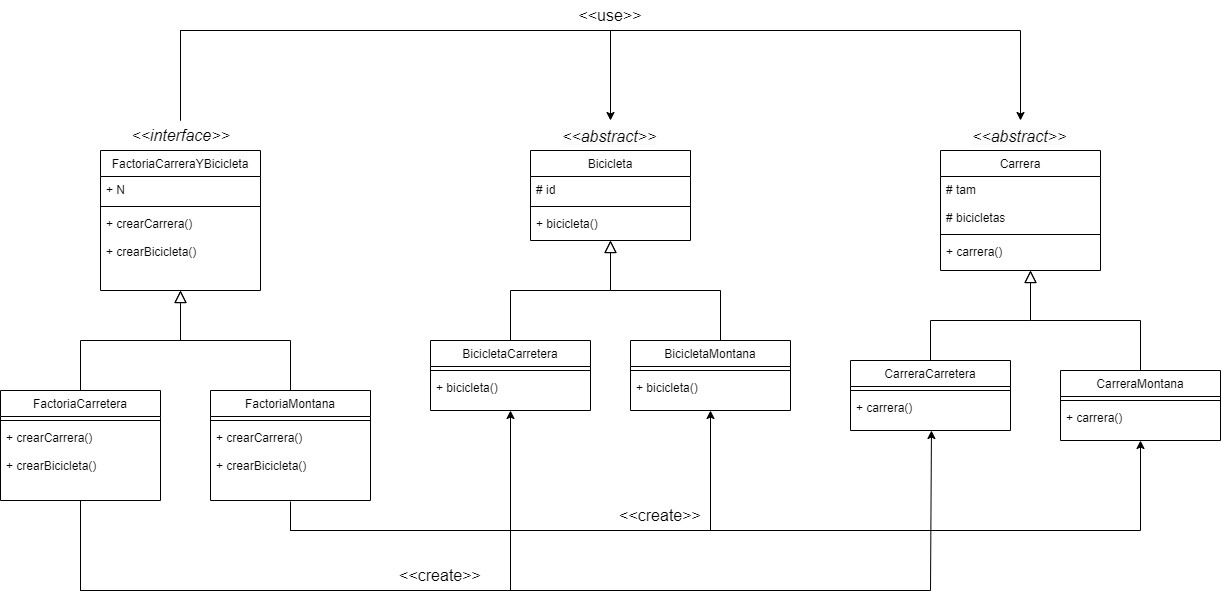
\includegraphics[width=\textwidth]{imagenes/Ejercicio 1.jpeg}

    \subsection{Resolución}
    \hspace*{1cm}Empezamos creando la \textit{interfaz FactoriaCarreraYBicicleta}, que define un contrato para una factoría abstracta que
    crea objetos relacionados con carreras y bicicletas. Los métodos que implementa son los siguientes:

    \begin{itemize}
        \item \textit{crearCarrera}: Mëtodo para crear un carrera. Devuelve una instancia de la clase Carrera.
        \item \textit{crearBicicleta}: Método para crear una bicicleta. Devuelve una instancia de la clase Bicicleta
    \end{itemize}

    \hspace*{1cm}La clase abstracta \textit{Bicicleta} proporciona una estructura base para representar bicicletas.
    Contiene un atributo \textbf{id}, tipo entero que es el identificador único de cada bicicleta.
    Tiene un método abstracto \textit{bicicleta()} que muestra la bicicleta, y será implementado por las clases concretas.\\
    
    \hspace*{1cm}La clase abstracta \textit{Carrera} proporciona una estructura base para representar carreras.
    Contiene un atributo \textbf{tam}, tipo entero que representa el número máximo de bicicletas que participan en la carrera,
    además de un ArrayList$<$Bicicleta$>$ \textbf{Bicicletas}, que almacena las bicicletas que participan en la carrera.
    Tiene un método abstracto \textit{carrera()} que muestra la carrera, y será implementado por las clases concretas.
    También tiene definido el constructor \textit{Carrera(tam)}, que recibe el tamaño de de la carrera. \\

    \hspace*{1cm}La clase \textit{BicicletaCarretera} representa una bicicleta diseñada específicamente para
    carreras de carretera. Implementa el método \textit{bicicleta()}, heredado de \textit{Bicicleta}, que muestra una bicicleta de carretera,
    e imprime un mensaje indicando que es una bici de carretera y su respectivo identificador. \\

    \hspace*{1cm}La clase \textit{BicicletaMontana} representa una bicicleta diseñada específicamente para
    carreras de montaña. Implementa el método \textit{bicicleta()}, heredado de \textit{Bicicleta}, que muestra una bicicleta de montaña,
    e imprime un mensaje indicando que es una bici de montaña y su respectivo identificador.\\
    
    \hspace*{1cm}La clase \textit{CarreraCarretera} representa un carrera específica que se lleva a cabo en carreteras.
    Implementa el método \textit{carrera()}, heredado de \textit{Carrera}, que muestra un carrera de carretera, 
    e imprime un mensaje indicando que es una carrera de carretera. También implementa el constructor \textit{CarreraCarretera(tam)}, 
    que recibe el tamaño de la carrera. \\

    \hspace*{1cm}La clase \textit{CarreraMontana} representa un carrera específica que se lleva a cabo en montañas.
    Implementa el método \textit{carrera()}, heredado de \textit{Carrera}, que muestra un carrera de montaña, 
    e imprime un mensaje indicando que es una carrera de montaña. También implementa el constructor \textit{CarreraMontana(tam)}, 
    que recibe el tamaño de la carrera. \\

    \hspace*{1cm}La clase \textit{FactoriaCarretera} implementa la intezfaz \textit{FactoriaCarreraYBicicleta} y proporciona métodos
    para crear carreras y bicicletas específicas para carreteras. Implementa los siguientes métodos:

    \begin{itemize}
        \item \textit{crearCarrera()}: Método para crear una carrera de carretera. Devuelve una instancia de la clase \textit{Carrera} 
                que representa una carrera de carretera.
                El método crea una instancia de CarreraCarretera con el tamaño N. 
                Agrega bicicletas a la carrera. 
                Calcula la cantidad de bicicletas a eliminar (10\%). 
                Genera una lista de índices aleatorios para bicicletas a eliminar. 
                Calcula la nueva longitud de la lista de bicicletas después de eliminar. 
                Crea una nueva carrera con la nueva longitud calculada. 
                Copia las bicicletas de la carrera original a la nueva carrera, omitiendo las eliminadas. 
                Actualiza la carrera con la nueva carrera.
        \item \textit{crearBicicleta()}: Método para crear una bicicleta de carretera. Devuelve un instancia de la clase \textit{Bicicleta}.
    \end{itemize}

    \hspace*{1cm}La clase \textit{FactoriaMontana} implementa la intezfaz \textit{FactoriaCarreraYBicicleta} y proporciona métodos
    para crear carreras y bicicletas específicas para montañas. Implementa los siguientes métodos:

    \begin{itemize}
        \item \textit{crearCarrera()}: Método para crear una carrera de montaña. Devuelve una instancia de la clase \textit{Carrera} 
                que representa una carrera de montaña.
                El método crea una instancia de CarreraMontana con el tamaño N. 
                Agrega bicicletas a la carrera. 
                Calcula la cantidad de bicicletas a eliminar (20\%). 
                Genera una lista de índices aleatorios para bicicletas a eliminar. 
                Calcula la nueva longitud de la lista de bicicletas después de eliminar. 
                Crea una nueva carrera con la nueva longitud calculada. 
                Copia las bicicletas de la carrera original a la nueva carrera, omitiendo las eliminadas. 
                Actualiza la carrera con la nueva carrera.
        \item \textit{crearBicicleta()}: Método para crear una bicicleta de montaña. Devuelve un instancia de la clase \textit{Bicicleta}.
    \end{itemize}

    \hspace*{1cm}La clase \textit{\textbf{main}}, que es el método principal del programa. Este método crea las factorías y 
    carreras para las carreras de montaña y de carretera, crea e inicia las hebras para ejecutar las carreras, y 
    luego espera a que las hebras terminen. Finalmente, imprime el número de bicicletas que completaron la carrera. \\
    También se crea la clase \textit{CarreraRunnable}, que implementa la interfaz Runnable y representa una hebra que ejecuta una carrera.
    Tiene definidos e implementados dos métodos:

    \begin{itemize}
        \item \textit{CarreraRunnable(Carrera carrera)}: Es el constructor de la clase, que recibe la carrera que la hebra va a ejecutar.
        \item \textit{run()}: Método que se ejecuta cuando se inicia la hebra. Este método hace que la hebra dure 60 segundos e imprima 
                el identificador de cada bicicleta que completó la carrera.
    \end{itemize}

    \section{Ejercicio 2}
    \subsection*{Enunciado}
    \hspace*{1cm}Diseña e implementa una aplicación con la misma funcionalidad que la del ejercicio anterior,
    pero que aplique el patrón \textit{Prototipo} junto con el patrón \textit{Factoría Abstracta}.\\
    \hspace*{1cm}Se elegirá el lenguaje de programación Python o Ruby. Para simplificar: no es necesario
    el uso de hebras.

    \subsection{Diagrama UML}
    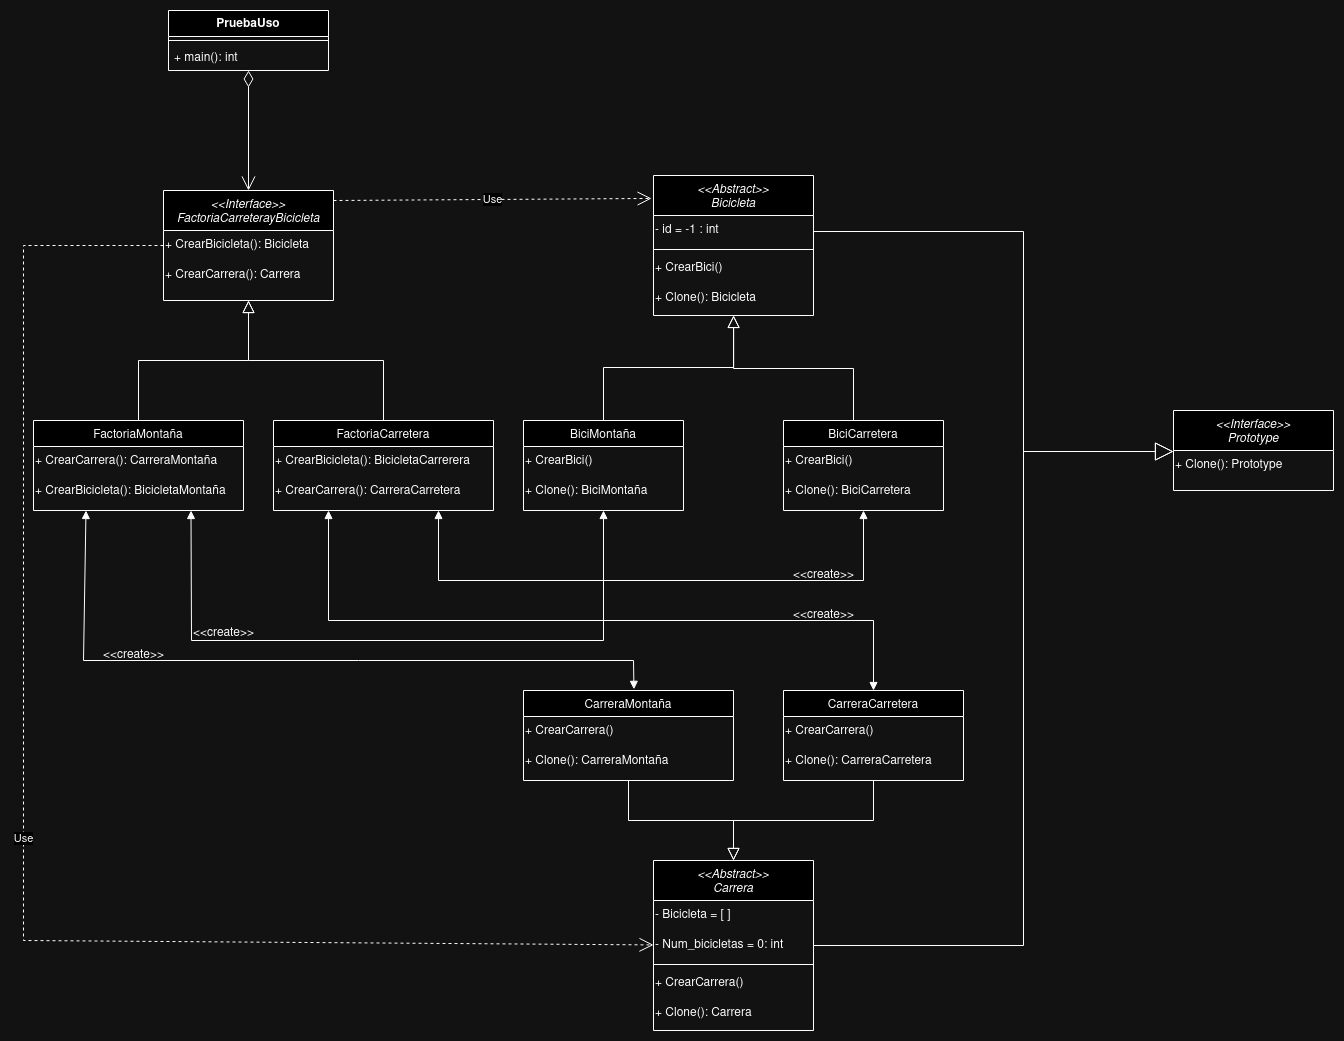
\includegraphics[width=\textwidth]{imagenes/P1-E2.drawio.png}

    \subsection{Resolución del ejercicio}

    \hspace*{1cm}La resolución de este ejercicio es muy parecida a la anterior, donde hemos creado una factoria \textit{interface}
    de carreras y bicicletas, de la que heredan las factorias de Montaña y de Carretera. \\
    Estas últimas, implementan varios métodos heredados de la clase \textit{interface}, llamados
    \textit{crearCarrera()} y \textit{crearBicicleta()}, donde en cada Factoria se creará un objeto diferente, bien sea 
    de montaña o de carretera. \\
    Por otro lado, tenemos dos clases $<<$\textit{abstract}$>>$: \textit{Bicicleta} y \textit{Carrera}, que definen
    un método para crear un objeto de la clase, que será implementado en las clases hijas, \textit{BiciMontaña}, 
    \textit{BiciCarretera}, \textit{CarreraMontaña} o \textit{CarreraCarretera}, creando así el objeto
    respectivo de montaña o de carretera.\\

    \hspace*{1cm}Para crear los objetos no es necesario que se haga uno a uno, sino que podemos crear únicamente el primero y a 
    partir de ese, clonar el resto. De este modo, hemos creado una clase \textit{interface Prototype} donde definimos un 
    método \textit{clone()} que heredarán \textit{Bicicleta} y \textit{Carrera}, que a la vez heredarán e implmentarán sus hijas.

    \section{Ejercicio 3}
    \subsection{Enunciado}
    \hspace*{1cm}Diseño e implementación de una aplicación que utilice un patrón de diseño libre.
    Hemos diseñado una aplicación que crea vehículos, desde sus ruedas y motor hasta la transmisión y el color. Para ello, hemos 
    decidido usar el patrón de diseño \textit{Builder}.

    \begin{itemize}
        \item Usar Patrón Builder o algún Patrón que NO sea creacional para no repetir.
        \item Se valorará complejidad del problema y solución acordada en grupo.
        \item Extra: Combinación de patrones.
    \end{itemize}

    \subsection{Diagrama UML}
    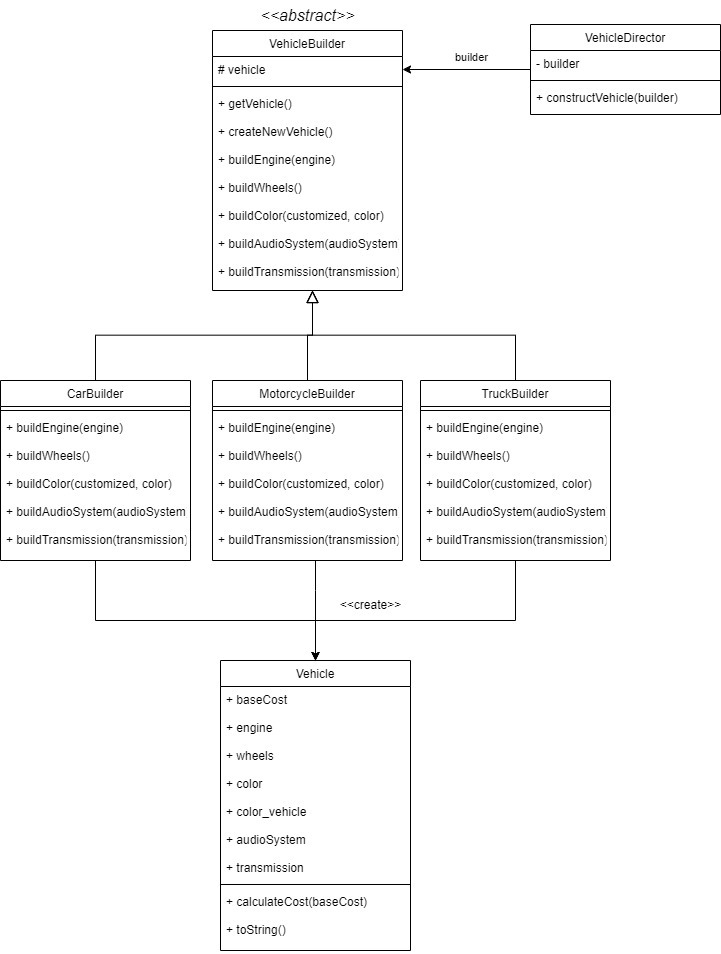
\includegraphics[width=\textwidth, height=\textheight]{imagenes/EJ3.jpeg}

    \subsection{Resolución}
    \hspace*{1cm}Empezamos creando la clase abstracta \textit{VehicleBuilder}, que define un contrado para construir vehículos,
    y nos permitirá contruir objetos complejos paso a paso.
    Contiene un atributo \textbf{vehicle} de tipo Vehicle, que representa el vehículo que se está construyendo.
    Los métodos que implementa son los siguientes:

    \begin{itemize}
        \item \textit{getVehicle()}: Método para obtener el vehículo construido. Devuelve el vehículo construido.
        \item \textit{createNewVehicle()}: Método para crear un nuevo vehículo. Crea una nueva instancia de Vehicle.
        \item \textit{buildENgine(engine)}: Método abstracto para construir el motor del vehículo. 
                El parámetro \textit{engine} indica el tipo de motor.
        \item \textit{buildWheels()}: Método abstracto para construir las ruedas del vehículo.
        \item \textit{buildColor(customized, color)}: Método abstracto para contruir el color del vehículo.
                El parámetro \textit{customized} indica si el color es personalizado o no.
                El parámetro \textit{color} indica el color del vehículo.
        \item \textit{buildAudioSystem(audioSystem)}: Método abstracto para construir el sistema del vehículo. 
                El parámetro audioSystem indica si el vehículo tiene sistema de audio o no.
        \item \textit{buildTransmission(transmission)}: Método abstracto para construir la transmisión del vehículo. 
                El parámetro transmission indica si el vehículo tiene transmisión o no.
    \end{itemize}

    \hspace*{1cm}La clase \textit{VehicleDirector} actúa como el director en el patrón \textit{Builder}. 
            Coordina el proceso de contrucción de un vehículo utilizando un \textbf{Vehicle Builder} específico. 
            Contiene el atributo \textit{builder}, de tipo VehicleBuilder, que se utilizará para construir el vehículo.
    Los métodos que implementan son:

    \begin{itemize}
        \item \textit{VehicleDirector(builder)}: Constructor de la clase. EL parámetro \textit{builder} es el constructor de vehículos a utilizar.
        \item \textit{constructVehicle()}: Método para construir el vehículo. 
                Coordina el proceso de construcción de un vehículo utilizando el constructor de vehículos especificado.
    \end{itemize}

    \hspace*{1cm}La clase \textit{CarBuilder} es una implementación concreta de \textit{VehicleBuilder} que se utiliza para contruir vehículos
    de tipo automóvil. Los métodos que implementa son:

    \begin{itemize}
        \item \textit{CarBuilder()}: Constructor de la clase. Crea una nueva instancia de \textit{CarBuilder} y llama al método 
                \textit{createNewVehicle()} para inicializar el nuevo vehículo.
        \item \textit{buildEngine(engine)}: Método para contruir el motor del automóvil. Devuelve el tipo de motor.
        \item \textit{buildWheels()}: Método para construir las ruedas del automóvil.
        \item \textit{buildColor(customized, color)}: Método para construir el color del automóvil.
                El parámetro customized indica si el color es o no personalizado.
                El parámetro colo indica el color del automóvil.
        \item \textit{buildAudioSystem(audioSystem)}: Método para construir el sistema de audio del automóvil. 
                El parámetro audioSystem indica si el automóvil tiene un sistema de audio o no.
        \item \textit{buildTransmission(transmisión)}: Método para construir la transmisión del automóvil. 
                El parámetro transmission indica si el automóvil tiene o no transmisión.
    \end{itemize}

    \hspace*{1cm}La clase \textit{MotorcycleBuilder} es una implementación concreta de \textit{VehicleBuilder} que se utiliza para contruir vehículos
    de tipo motocicleta. Los métodos que implementa son:

    \begin{itemize}
        \item \textit{MotorcycleBuilder()}: Constructor de la clase. Crea una nueva instancia de \textit{MotorcycleBuilder} y llama al método 
                \textit{createNewVehicle()} para inicializar el nuevo vehículo.
        \item \textit{buildEngine(engine)}: Método para contruir el motor de la motocicleta. Devuelve el tipo de motor.
        \item \textit{buildWheels()}: Método para construir las ruedas de la motocicleta.
        \item \textit{buildColor(customized, color)}: Método para construir el color de la motocicleta.
                El parámetro customized indica si el color es o no personalizado.
                El parámetro colo indica el color de la motocicleta.
        \item \textit{buildAudioSystem(audioSystem)}: Método para construir el sistema de audio de la motocicleta. 
                El parámetro audioSystem indica si la motocicleta tiene un sistema de audio o no.
        \item \textit{buildTransmission(transmisión)}: Método para construir la transmisión de la motocicleta. 
                El parámetro transmission indica si la motocicleta tiene o no transmisión.
    \end{itemize}

    \hspace*{1cm}La clase \textit{TruckBuilder} es una implementación concreta de \textit{VehicleBuilder} que se utiliza para contruir vehículos
    de tipo camión. Los métodos que implementa son:

    \begin{itemize}
        \item \textit{TruckBuilder()}: Constructor de la clase. Crea una nueva instancia de \textit{TruckBuilder} y llama al método 
                \textit{createNewVehicle()} para inicializar el nuevo vehículo.
        \item \textit{buildEngine(engine)}: Método para contruir el motor del camión. Devuelve el tipo de motor.
        \item \textit{buildWheels()}: Método para construir las ruedas del camión.
        \item \textit{buildColor(customized, color)}: Método para construir el color del camión.
                El parámetro customized indica si el color es o no personalizado.
                El parámetro colo indica el color de la motocicleta.
        \item \textit{buildAudioSystem(audioSystem)}: Método para construir el sistema de audio del camión. 
                El parámetro audioSystem indica si el camión tiene un sistema de audio o no.
        \item \textit{buildTransmission(transmisión)}: Método para construir la transmisión del camión. 
                El parámetro transmission indica si el camión tiene o no transmisión.
    \end{itemize}

    \hspace*{1cm}La clase \textit{Vehicle} representa un vehículo y proporciona métodos para calcular su costo y representarlo como una cadena de texto.
    Los atributos que posee son:

    \begin{itemize}
        \item \textbf{baseCost}(double): Indica el costo base del vehículo.
        \item \textbf{engine}(string): Indica el tipo de motor del vehículo.
        \item \textbf{wheels}(int): Indica el número de ruefas del vehículo.
        \item \textbf{color}(boolean): Indica si el color del vehículo es personalizado (true) o no (false);
        \item \textbf{color\_vehicle}(string): Indica el color de vehículo.
        \item \textbf{audioSystem}(boolean): Indica si el vehículo tiene sistema de audio (true) o no (false);
        \item \textbf{transmisión}(boolean): Indica si el vehículo tiene transmisión personalizada (true) o no (false);   
    \end{itemize}

    Los métodos que implementa son:

    \begin{itemize}
        \item \textit{calculateCost(baseCost)}: Método para calcular el costo total del vehículo. El parámetro \textbf{baseCost} indica el costo base del vehículo.
                Devuelve el costo total del vehículo, incluido los costos adicionales por características personalizadas.
        \item \textit{toString()}: Método para representar el vehículo como una cadena de texto.
                Devuelve una cadena de texto que representa al vehículo.
    \end{itemize}

    \hspace*{1cm}La clase \textit{\textbf{main}} es la clase principal del programa, que interactúa con el usuario para 
    configurar y construir vehículos personalizados.\\
    
    \hspace*{1cm}El método pedirá al usuario que elija el tipo de vehículo. A continuación, solicitará información específica
    del vehículo, como el tipo de motor, el color, la transmisión y el sistema de audio. Finalmente, construye el vehículo, 
    muestra la información dle vehículo y calcula su costo total.



    \newpage

    \section{Ejercicio 4}
    \subsection{Diagrama UML}
    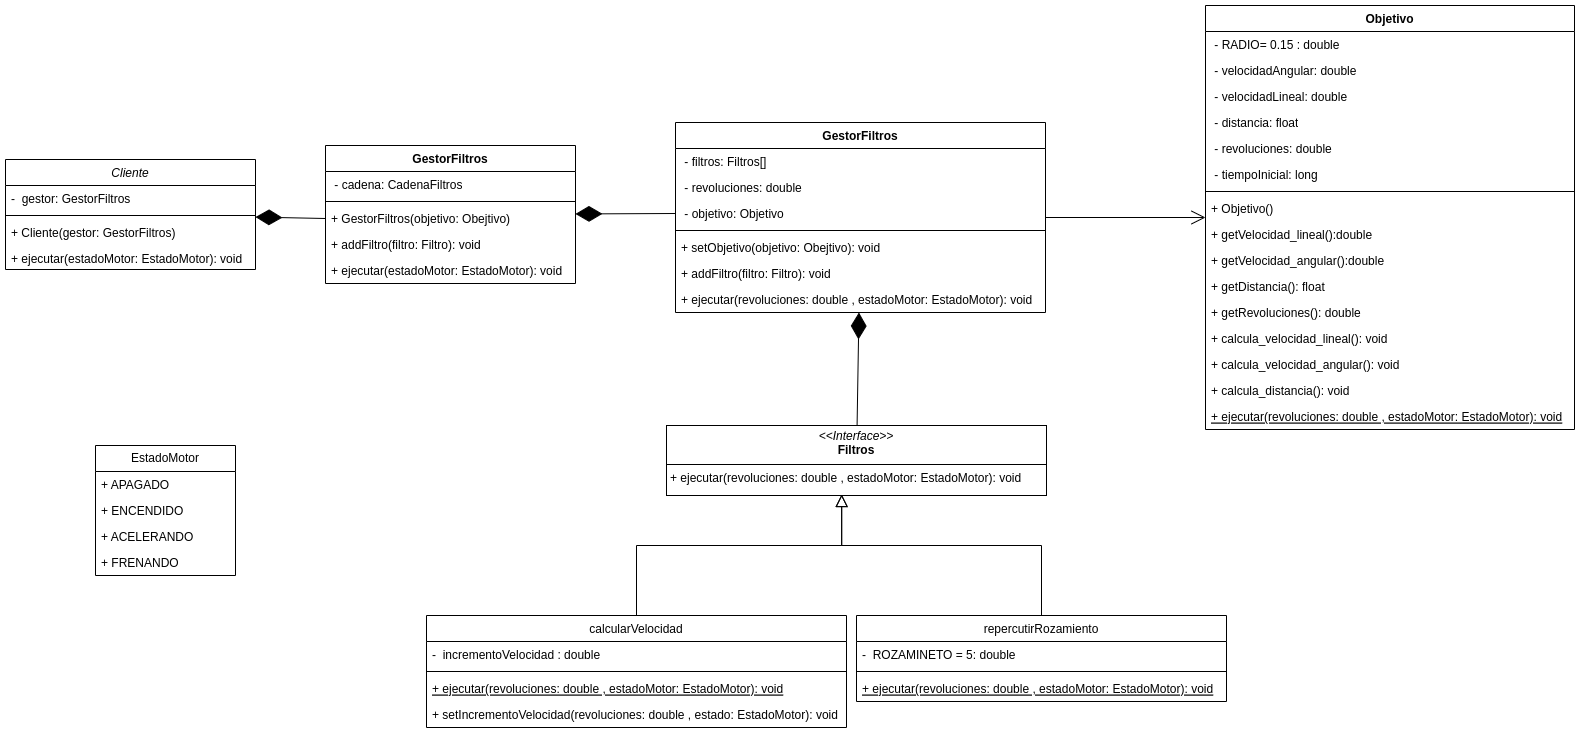
\includegraphics[width=\textwidth]{imagenes/Ej4_Practica1_DS.png}

    \subsection{Resolución}
    \hspace*{1cm}Empezaremos creando la clase \textit{Cliente}, que representará un cliente que utiliza un \textbf{GestorFiltros}
    para establecer las revoluciones del motor apartir de un estado que se le pase. La clase tiene el atributo \textbf{gestor}, que
    indica el gestor de filtros utilizado por el cliente.
    Los métodos de la clase son:

    \begin{itemize}
        \item \textit{Cliente(GestorFiltros g)}: Constructor de la clase que recibe un gestor de filtros como parámetroy lo asigna
                al atributo \textbf{gestor}.
        \item \textit{ejecutar(EstadoMotor estadoMotor)}: Método que ejecuta los filtros en el motor utilizando el gestor de filtros
                asignado. El parámetro que recibe es el estado actual del motor.
    \end{itemize}

    \hspace*{1cm}La clase \textit{GestorFiltros} gestiona una cadena de filtros y proporciona métodos para agregar filtros y ejecutarlor
    en un motor. Tiene un atributo \textbf{cadena} que indica la cadena de filtros suministrada por el gestor.
    Define los siguiente métodos:

    \begin{itemize}
        \item \textit{GestorFiltros(Objetivo o)}: Constructor de la clase que recibe un objetivo como parámetro sobre el que se
                aplicarán los filtros y que se pasará a \textbf{CadenaFiltros}.
        \item \textit{addFiltro(Filtro f)}: Agrega un filtro a la cadena de filtros suministrada por el gestor.
        \item \textit{ejecutar(EstadoMotor estadoMotor)}: Ejecuta la cadena de filtros en el motor.
                El parámetro \textit{estadoMotor} indica el estado actual del motor.
    \end{itemize}

    \hspace*{1cm}La clase \textit{CadenaFiltros} gestiona una lista de filtros y proporciona métodos para agregar filtros, 
    establecer un objetivo y ejecutar los filtros en un motor. Los atributos de la clase son:

    \begin{itemize}
        \item \textbf{filtros}: Una lista de filtros.
        \item \textbf{objetivo}: El objetivo al que se aplicarán los filtros.
        \item \textbf{revoluciones}: Las revoluciones actuales del motor.
    \end{itemize}

    Los métodos que implementa son:

    \begin{itemize}
        \item \textit{addFiltro(Filtro f)}: Agrega un filtro a la lista de filtros.
        \item \textit{setObjetivo(Objetivo o)}: Establece el objetivo al que se aplicarán los filtros.
        \item \textit{ejecutar(EStadoMotor estadoMotor)}: Ejecuta la lista de filtros en el motor y, opcionalmente, ejecuta el objetivo.
    \end{itemize}

    \hspace*{1cm}La clase interfaz \textit{Filtro} define el método \textit{ejecutar(double revoluciones, EstadoMotor estadoMotor)} 
    para ejecutar filtros en un motor, donde \textbf{revoluciones} son las revoluciones actuales del motor y \textbf{estadoMotor}
    el estado actual del motor, y que devuelve el resultado de aplicar el filtro (double);

    \hspace*{1cm}La clase \textit{FiltroCalcularVelocidad} implementa la interfaz \textit{Filtro} y proporcionar métodos Para
    calcular la velocidad de un motor.
    Los atributos de la clase son:

    \begin{itemize}
        \item \textbf{incrementoVelocidad}: Parámetro que indica el cambio de velocidad.
        \item \textbf{MAX\_REVOLUCIONES}: Representa el máximo de revoluciones permitidas antes de ajustar la velocidad.
    \end{itemize}

    Los métodos que implementa son:

    \begin{itemize}
        \item \textit{setIncrementoVelocidad(double revoluciones, EstadoMotor estado)}: Establece el incremento de velocidad según las
                revoluciones y el estado del motor, en caso de que las revoluciones sean mayores que \textbf{MAX\_REVOLUCIONES} hace que
                el \textbf{incrementoVelocidad} sea 0.
        \item \textit{ejecutar(double revoluciones, EstadoMotor estadoMotor)}: Calcula la velocidad del motor en función de las revoluciones
                y el estado del motor, y devuelve nuevo valor para las revoluciones de motor. En caso de ser menor que 0, devuelve \textbf{revoluciones} = 0.
    \end{itemize}

    \section{Ejercicio 5}
    \subsection{Enunciado}
    \hspace*{1cm}Diseño de una aplicación de WebScraping en Python donde se utilice el Patrón Strategy
    para scrapear información en vivo de acciones en la página web \textit{\textbf{https://finance.yahoo.com/quote/}}, 
    donde se puede añadir el sufijo de la acción para acceder a información en vivo de ésta. \\
    Ejemplo con TESLA: \textit{\textbf{https://finance.yahoo.com/quote/TSLA}}.
    
    \subsection{Diagrama UML}
    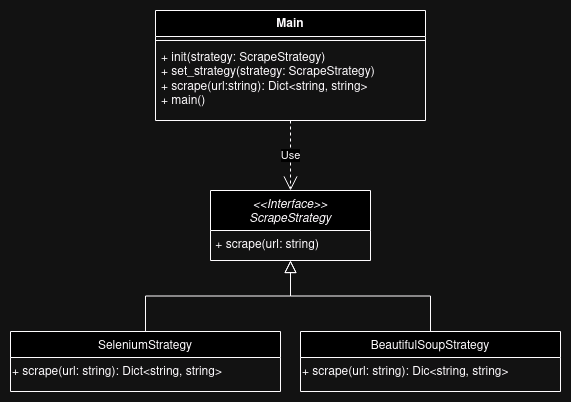
\includegraphics[width=\textwidth]{imagenes/P1_E5.drawio.png}
    
    \subsection{Resolución}
    \hspace*{1cm}Empezamos con la clase interfaz \textit{Scraper}, que contendrá la definición de la función
    \textit{scrape(self, url)}, que estará implementada en las clases hijas \textit{Selenium} y \textit{BeautifulSoup}.

    \hspace*{1cm}La clase \textit{BeautifulSoup} implementa el método \textit{scrape(self, url)}, que se encarga de acceder 
    a la url que le pasamos como parámetro. Realizamos un GET a la url. Verificamos si tuvimos exito en la operación 
    si el código de estado es 200 (OK). Si tuvimos exito, procedemos a estraer los datos de la página web, de lo contrario,
    devuelve un mensaje de error diciendo que no pudimos obtener la página. Si la solicitud fue exitosa, creamos un objeto 
    BeautifulSoup y procedemos a encontrar los elementos buscados con el método de búsqueda \textit{find()}.\\
    Los datos serán almacenados en un diccionario, que será devuelto como resultado de la función.

    \hspace*{1cm}La clase \textit{Selenium} implementa el método \textit{scrape}, que se configura para utilizar el navegador 
    Chrome en modo \textit{\textbf{sin cabeza}} (headless), para que el navegador se ejecute en segundo plano sin mostrar
    interfaz gráfica, mejorando la velocidad en el proceso de scrapeo.\\
    Luego el navegador accede a la página de las acciones de Tesla en Yahoo Finance utilizando la url y espera hasta que 
    el botón de aceptar cookies sea detectable para hacer el click. Después de esto, utilizando la clase \textit{WebDriverWait}, 
    se establece un periodo de espera explícito para cada elemento que queremos leer mediante su \textbf{XPATH} específico. De 
    esta manera se asegura que el script haga una espera adecuada para que los elementos estén presentes en la página antes de 
    intentar acceder a sus datos.\\
    Una vez extraidos los datos se cierra el navegador limpiamente para asegurar que no queden procesos ejecutándose en segundo plano.


    \hspace*{1cm}En la clase \textit{\textbf{main}} crearemos un dato llamado \textbf{url}, que contendrá la url de la página
    web que queremos scrapear. Llamaremos al constructor de la clase, que recibe una estrategia. Luego, llamaremos al método
    \textit{scrape(url)}, que llamará al método \textit{scrape(url)} del objeto estrategia, y almacenará el resultado en la 
    variable \textbf{data}, que contendrá el diccionario de los elementos buscados. \\
    Por último, imprimiremos los valores encontrados y los añadiremos a un archivo json llamado \textit{\textbf{data.json}}.

\end{document}
